\documentclass[../report.tex]{subfiles}
\begin{document}	
	
\chapter{Fabrication}
To test the \gls{tpr} it is necessary to design auxiliary components like grating couplers (\gls{te} \& \gls{tm}), tapers, \gls{pbs}. The gratings are designed in way to couple \gls{te} and \gls{tm}-modes from the LASER to the waveguide taper. The tapers are connected to the \gls{tpr}, to direct the light into it. Finally, a \gls{pbs} is designed which again decouples the \gls{te} and \gls{tm}-modes to the grating couplers via tapers where a photo-detector measures the intensity of output modes.  

\begin{figure}[H] %h
	\centering
	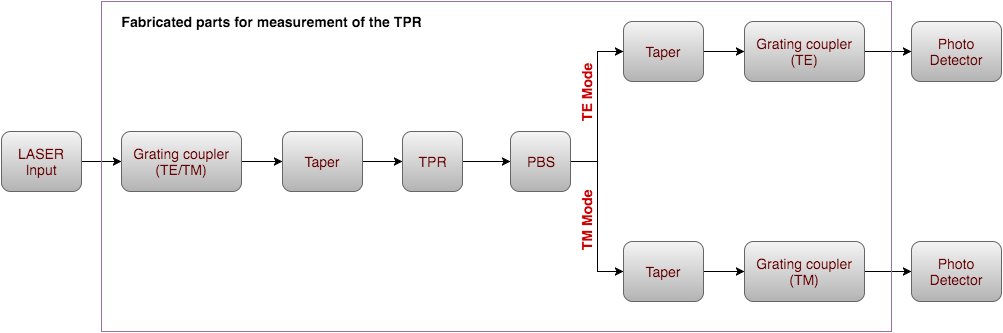
\includegraphics[width=1\textwidth]{4-sys-design}
	\caption{System level block diagram of the fabricated device}
	\label{fig:4_sys_design}
\end{figure}

\section{Process}
The \gls{mems} tunable device was fabricated using a SOI-based process with two dry etch steps for the silicon device layer (resulting in two heights) and a wet $SiO_2$ under-etch \cite{errando-herranz_low-power_2015}. The first lithography step defines the ridge waveguides that form the ring resonator and the grating coupled bus waveguide. \todo{Update with my process thing} The second lithography step and the wet under-etch define the free standing cantilever. The cantilever is delimited by the fully etched slot waveguides, and its free suspended area is determined by the placement of etch holes.

\par The fabrication process starts with a clean SOI chip with a \SI{220}{\nano \meter} crystalline silicon device layer and \SI{2}{\micro \meter} buried oxide (\ref{fig:4_fabrication} A). This is a standard substrate specification used by the Epixfab silicon photonics foundries. Electron beam patterning of a \SI{50}{\nano \meter} layer of a high-resolution negative electron beam resist (\gls{hsq}) defines the waveguide structures (\ref{fig:4_fabrication} B). The pattern is then transferred to the device layer by timed dry etch of silicon, resulting in ridge waveguide structures with \SI{110}{\nano \meter} height on a \SI{110}{\nano \meter} thick silicon slab ((\ref{fig:4_fabrication} C)). The patterned \gls{hsq} remains on the chip for the next lithography step.

\begin{figure}[H] %h
	\centering
	\includegraphics[width=0.5\textwidth]{4-fabrication}
	\caption{Fabrication process}
	\label{fig:4_fabrication}
\end{figure} \todo{Update E,F,G}

Unit Test
Same strategy as Software unit test
1. Test if a normal waveguide with TE-TE grating is working with taper.
2. Test if a normal waveguide with TE-TM grating is working with taper.
3. Test if a normal waveguide with TM-TE grating is working with taper.
4. Test if a normal waveguide with TM-TM grating is working with taper.
4. Test if a normal waveguide with PBS TE/TM-TM/TE grating is working with taper.
5. Test if PR waveguide works with PBS and TE/TM grating for different lengths with taper.
6. Check if a normal cantilever is working and it does not stick.
7. Check actuation using separation strategy.
8. 

1. Pirahna bath - SOI cleaning
2. HSQ spin (negative resist) - Check profile for depth of mask
3. E-beam (HSQ hardening - pattern drawing). No alignment problem as it is a fresh chip. Focus correction to avoid beam deflection too much. Focus correction is done using scratching a portion of the chip and then exposing it using e-beam. Why not expose the whole chip and do focus correction? - Since, since e-beam shoots electrons it can over-expose the patterns and the resolution will also not be fine.
4. Curing of non-hardened HSQ in solvent (name?)
5. Initially the dry etch chamber is seasoned with a seasoning wafer. Chlorine ion, HBr ion (H+, Br-) etch of Silicon. Check Silicon profile. Etch depth profile according to the gas ion exposure time.
6. ZEP7000 spin (positive resist) - Check profile for depth of mask
7. E-beam of ZEP. Now alignment has to be done each time to expose e-beam correctly. Alignement is done using 3 marks on the chip and each sub-section of the chips where the test cases are examined. This is needed in the second e-beam as we need to know exactly where the mask should be softened in accordance with the previous e-beam step with HSQ.
8. Curing of e-beamed ZEP. Since positive resist, the exposed portions become dissolved Isopropanol solvent.





\section{Final Product}

Show SEM image

\end{document}
